% begin module maclaurin-series-def
\begin{frame}
Suppose we wanted to find a fourth degree polynomial of the form:
\[
P(x)=a_0+a_1x+a_2x^2+a_3x^3+a_4x^4
\]
that approximates the behaviour of a transcendental function such as, say $ f(x)=\ln(x+1) $ near $ x=0. $\\

 \pause
If we make $P(0)=f(0) $, and ensure the first, second, third and fourth derivatives are the same, then we would have a pretty good approximation.

\end{frame}
% end module maclaurin-series-def

\begin{frame}
\frametitle{ $ f(x)=\ln(x+1) $, $ P(x)=a_0+a_1x+a_2x^2+a_3x^3+a_4x^4 $}

\[
\left. \begin{array}{ll}
\uncover<2->{f(x)=\ln(x+1)}     & \uncover<2->{P(x)=a_0+a_1x+a_2x^2+a_3x^3+a_4x^4}\\
\uncover<3->{f(0) = \ln(1) = 0 } & \uncover<4->{P(0)=a_0}\\
\end{array}
\right\}
\uncover<5->{\Rightarrow \alert<5>{a_0=0}}
\]
\[
\left.
\begin{array}{ll}
\uncover<6->{f'(x)=\frac{1}{x+1}}     & \uncover<6->{P'(x)= a_1 +2a_2x +3a_3x^2+4a_4x^3}\\
\uncover<7->{f'(0) = 1 } & \uncover<8->{P'(0)=a_1}\\
\end{array}
\right\}
\alert<9>{\uncover<9->{\Rightarrow a_1=1}}
\]
\[
\left.
\begin{array}{ll}
\uncover<10->{f''(x)=-\frac{1}{(x+1)^2}}     & \uncover<10->{P''(x)=2a_2 +6a_3x +12a_4x^2}\\
\uncover<11->{f''(0) = -1 } & \uncover<11->{P''(0)=2a_2}\\
\end{array}
\right\}
\alert<12>{\uncover<12->{\Rightarrow a_2=-\frac12}}
\]

\[
\left.
\begin{array}{ll}
\uncover<13->{f^{(3)}(x)= \frac{2}{(x+1)^3}}     & \uncover<13->{P^{(3)}(x)= 6a_3  +24a_4x }\\
\uncover<14->{f^{(3)}(0) = 2 } & \uncover<14->{P^{(3)}(0)=6a_3}\\
\end{array}
\right\}
\alert<15>{\uncover<15->{\Rightarrow a_3=\frac26}}
\]

\[
\left.
\begin{array}{ll}
\uncover<16->{f^{(4)}(x)= -\frac{6}{(x+1)^4}}     & \uncover<16->{P^{(4)}(x)=  24a_4  }\\
\uncover<17->{f^{(4)}(0) = -6 } & \uncover<17->{P^{(4)}(0)=24a_4}\\
\end{array}
\right\}
\alert<18>{\uncover<18->{\Rightarrow a_4=-\frac{6}{24}}}
\]
\[
 P(x)= \only<1-4>{a_0} \alert<5>{\only<5->{0}}+\only<1-8>{a_1}\alert<9>{\only<9->{1}} x+\only<1-11>{a_2} \alert<12>{\only<12->{-\frac12}}x^2+\only<1-14>{a_3} \alert<15>{\only<15->{\frac26}}x^3+\only<1-17>{a_0} \alert<18>{\only<18->{-\frac{6}{24}}}x^4 
\]


\end{frame}
% end module maclaurin-series-def

\begin{frame}

\begin{tikzpicture}
\begin{axis}[ 
	xmin=-2, xmax=2,
	ymin=-3, ymax=3,
	xtick={-2,...,2}, ytick={-3,...,3},
	major tick length={5},
	line width=1pt,
	axis lines=center
	] 
	\addplot[blue,smooth,domain=-0.95:2] {ln(x+1)};
	\only<2>{\addplot[red,smooth,domain=-2:2] {0};}
	\only<3>{\addplot[red,smooth,domain=-2:2] {0+x};}
	\only<4>{\addplot[red,smooth,domain=-2:2] {0+x-(x^2)/2};}
 	\only<5>{\addplot[red,smooth,domain=-2:2] {0+x-(x^2)/2+(x^3)/3};}
 	\only<6->{\addplot[red,smooth,domain=-2:2] {0+x-x^2/2+(x^3)/3-(x^4)/4};}
 	\only<3->{\addplot[gray,smooth,thin,domain=-2:2] {0};}
 	\only<4->{\addplot[gray,smooth,thin,domain=-2:2] {0+x};}
 	\only<5->{\addplot[gray,smooth,thin,domain=-2:2]{0+x-(x^2)/2};}
 	\only<6->{\addplot[gray,smooth,thin,domain=-2:2] {0+x-(x^2)/2+(x^3)/3};}
\end{axis}
\end{tikzpicture}
\[
 P(x)= \only<2->{ 0 \only<3->{+ x \only<4->{-\frac12x^2 \only<5->{+\frac26 x^3 \only<6->{-\frac{6}{24} x^4}}}}} 
\]
We see that near zero the functions match very well!\\
Moreover, as the number of terms increases, we get better approximations.


\end{frame}
% end module maclaurin-series-def

\begin{frame}
Our polynomial approximation of $ \ln(x+1) $ \[
 P(x)= 0+ x  -\frac12x^2  +\frac26 x^3  -\frac{6}{24} x^4 
\]
has the form 
\[
f(0) + \frac{f'(0)}{1!}x + \frac{f''(0)}{2!}x^2 + \frac{f'''(0)}{3!}x^3 + + \frac{f^{(4)}(0)}{4!}x^4
\]
\pause 
This pattern occurs no matter what the original function was!\\
\pause 
In fact, if we had approximated $ f(x) $ near $ x=a $, instead of $ x=0 $, we would obtain the polynomial
\[
T_n(x) = f(a) + \frac{f'(a)}{1!}(x-a) + \frac{f''(a)}{2!}(x-a)^2 + \frac{f'''(a)}{3!}(x-a)^3 + + \frac{f^{(4)}(a)}{4!}(x-a)^4
\]
\pause 
\begin{definition}[Taylor and Maclauren Polynomials]
$ T_n $ is the $ n $'th degree \textbf{Taylor Polynomial} for $ f(x) $ (centered) at $ x=a $. If $ a=0 $, we obtain the $ n $'th degree \textbf{Maclauren Polynomial} for $ f $. For $ x $ ``near  $ a $" we have $ f(x) \approx T_n $ where
\abovedisplayskip=0pt
\belowdisplayskip=0pt
\[
T_n= \sum_{k=0}^n \frac{f^{(k)}(a)}{k!}(x-a)^k = f(a)+ \frac{f'(a)}{1!}(x-a) + \frac{f''(a)}{2!}(x-a)^2   + \cdots +\frac{f^{(n)}(a)}{n!}(x-a)^n%
\]
\end{definition}



\end{frame}
% end module maclaurin-series-def

\begin{frame}
 Continuing inductively, we obtain the Taylor and Maclauren Series' 

\begin{definition}[Taylor and Maclaurin Series]
The Taylor series of $f$ centered at $ a $ is the series
\abovedisplayskip=0pt
\belowdisplayskip=0pt
\begin{align*}
f(x) & = \sum_{n=0}^\infty \frac{f^{(n)}(a)}{n!}(x-a)^n\\ 
& = f(a) + \frac{f'(a)}{1!}(x-a) + \frac{f''(a)}{2!}(x-a)^2 + \frac{f'''(a)}{3!}(x-a)^3 + \cdots%
\end{align*}\pause 
The Maclaurin series of $f$ is the Taylor series of $f$ centered at $a = 0$.  In other words, it is the series
\abovedisplayskip=0pt
\belowdisplayskip=0pt
\begin{align*}
f(x) &= \sum_{n=0}^\infty \frac{f^{(n)}(0)}{n!}x^n\\
& = f(0) + \frac{f'(0)}{1!}x + \frac{f''(0)}{2!}x^2 + \frac{f'''(0)}{3!}x^3 + \cdots%
\end{align*}
\end{definition}
Note: These series might only converge (to $ f(x) $) for a "small" subset of $ \R $ near $ x=a $. 
\end{frame}
% end module maclaurin-series-def